\documentclass[compress]{beamer}
\usepackage{ifthen,verbatim,ulem}

\newcommand{\isnote}{}
\xdefinecolor{lightyellow}{rgb}{1.,1.,0.25}
\xdefinecolor{darkblue}{rgb}{0.1,0.1,0.7}

%% Uncomment this to get annotations
%% \def\notes{\addtocounter{page}{-1}
%%            \renewcommand{\isnote}{*}
%% 	   \beamertemplateshadingbackground{lightyellow}{white}
%%            \begin{frame}
%%            \frametitle{Notes for the previous page (page \insertpagenumber)}
%%            \itemize}
%% \def\endnotes{\enditemize
%% 	      \end{frame}
%%               \beamertemplateshadingbackground{white}{white}
%%               \renewcommand{\isnote}{}}

%% Uncomment this to not get annotations
\def\notes{\comment}
\def\endnotes{\endcomment}

\setbeamertemplate{navigation symbols}{}
\setbeamertemplate{headline}{\mbox{ } \hfill
\begin{minipage}{5.5 cm}
\vspace{-0.75 cm} \small
\end{minipage} \hfill
\begin{minipage}{4.5 cm}
\vspace{-0.75 cm} \small
\begin{flushright}
\ifthenelse{\equal{\insertpagenumber}{1}}{}{Jim Pivarski \hspace{0.2 cm} \insertpagenumber\isnote/\pageref{numpages}}
\end{flushright}
\end{minipage}\mbox{\hspace{0.2 cm}}\includegraphics[height=1 cm]{../cmslogo} \hspace{0.1 cm} \includegraphics[height=1 cm]{../tamulogo} \hspace{0.01 cm} \vspace{-1.05 cm}}

\begin{document}
\begin{frame}
\vfill
\begin{center}
\textcolor{darkblue}{\Large CSC Overlaps Alignment: Review and Conclusions}

\vfill
\begin{columns}
\column{0.3\linewidth}
\begin{center}
\large
\textcolor{darkblue}{Jim Pivarski}

\vspace{0.2 cm}
Alexei Safonov
\end{center}

\column{0.3\linewidth}
\begin{center}
\large
K\'aroly Banicz
\end{center}

\column{0.3\linewidth}
\begin{center}
\large
Jim Bellinger
\end{center}
\end{columns}

\begin{columns}
\column{0.3\linewidth}
\begin{center}
\scriptsize
{\it Texas A\&M University}
\end{center}

\column{0.3\linewidth}
\begin{center}
\scriptsize
{\it US-CMS}
\end{center}

\column{0.3\linewidth}
\begin{center}
\scriptsize
{\it University of Wisconsin}
\end{center}
\end{columns}

\vfill
30 October, 2008

\end{center}
\end{frame}

%% \begin{notes}
%% \item This is the annotated version of my talk.
%% \item If you want the version that I am presenting, download the one
%% labeled ``slides'' on Indico (or just ignore these yellow pages).
%% \item The annotated version is provided for extra detail and a written
%% record of comments that I intend to make orally.
%% \item Yellow notes refer to the content on the {\it previous} page.
%% \item All other slides are identical for the two versions.
%% \end{notes}

\small

\begin{frame}
\frametitle{Disclaimer}
\begin{itemize}\setlength{\itemsep}{0.35 cm}

\item We'll be talking about a discrepancy that we've previously
  described as an indication of an error in our track-based alignment

\item Since then, we've significantly cleaned up the analysis,
  understanding and correcting track-based errors, and the
  discrepancy has reduced by a factor of 3

\item By comparing final alignment results with photogrammetry, we
  have very strong circumstantial evidence that the remaining
  discrepancy is not due to misalignment or track-based issues

\item We have two remaining hypotheses that we propose here to get
  expert input.  If what we're suggesting is not possible, given what
  is known about the chamber geometry, then we (collectively) will
  have to scratch these out and find another explanation

\end{itemize}
\end{frame}

\begin{frame}
\frametitle{Outline for this talk}

\begin{itemize}\setlength{\itemsep}{0.5 cm}
\item Motivation and overview of the CSC Overlaps procedure
\item Developments since CMS Week, including
\begin{itemize}\setlength{\itemsep}{0.1 cm}
\item narrow and uniform residuals distributions
\item agreement with photogrammetry at the level of 300~$\mu$m
\end{itemize}
\item However, the ring still doesn't close (the ``discrepancy'' from page 1)
\item Conclusions: what might be causing the lack of closure, and \\ what has been ruled out
\end{itemize}

\end{frame}

\begin{frame}
\frametitle{Motivation for CSC Overlaps}
\begin{itemize}
\item Baseline alignment procedure shown to require 10--100~pb$^{-1}$ for a few hundred micron precision
\item Quicker alternative:
\begin{itemize}\setlength{\itemsep}{0.1 cm}
\item relative alignment of chambers in each ring (CSC Overlaps)
\item align whole ring relative to tracker with $\sim$1000s of \mbox{quality tracks\hspace{-1 cm}}
\end{itemize}
\item Can be done with CRAFT data
\end{itemize}

\begin{columns}
\column{0.5\linewidth}
Overlaps procedure:
\begin{enumerate}\setlength{\itemsep}{0 cm}
\item select tracks that pass through overlap of chambers in a ring
\item require consistency in pair of segments: slope and intercept
\item solve system
\end{enumerate}

\column{0.2\linewidth}
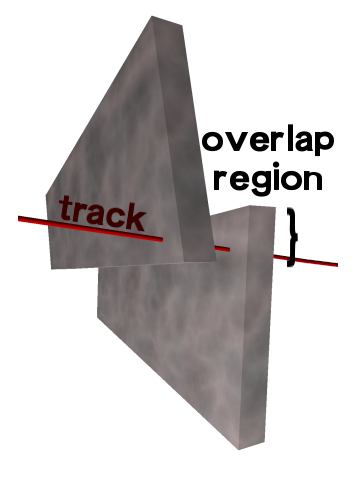
\includegraphics[width=\linewidth]{overlaps.png}

\column{0.3\linewidth}
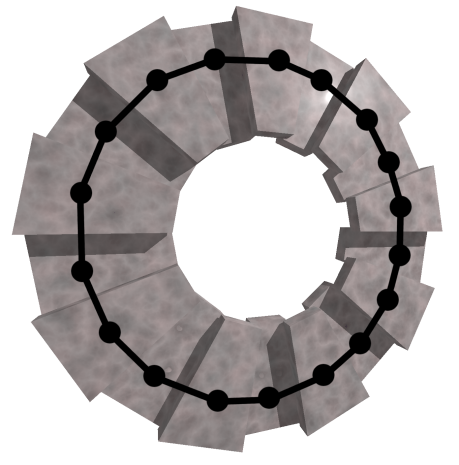
\includegraphics[width=\linewidth]{one_station.png}
\end{columns}

\vfill
System is over-constrained: must be consistent with a circle (``closure'')
\end{frame}

\begin{frame}
\frametitle{Details of implementation}

\begin{itemize}
\item Select good tracks, refit segments to 1-D straight \mbox{lines: $\phi(z) = a + b z$\hspace{-1 cm}}
\item Align $\varphi_y$ angles by requiring segments to have equal \mbox{slopes ($\Delta b = 0$)\hspace{-1 cm}}

\begin{center}
\begin{columns}
\column{0.45\linewidth}
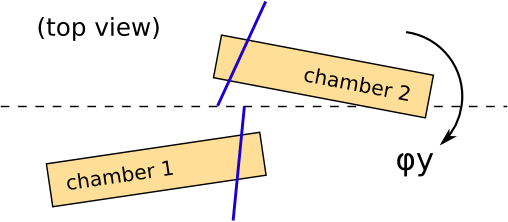
\includegraphics[width=\linewidth]{topview_1.png}
\column{0.01\linewidth}
\hfill $\to$ \hfill
\column{0.45\linewidth}
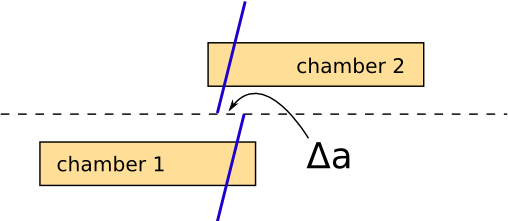
\includegraphics[width=\linewidth]{topview_2.png}
\end{columns}
\end{center}

\item Now intercept residual ($\Delta a$) tells us about misalignment in the $r\phi$ direction: align $\phi$ positions with fixed $r$ \mbox{(arcs centered on beamline)\hspace{-1 cm}}

\item Linear trend in intercept residual versus \\ radial position is due to $\varphi_z$ misalignment
\end{itemize}

\vspace{-1 cm}
\begin{columns}
\column{0.65\linewidth}

\vspace{0.4 cm}
Parameters decouple when corrected in this order: first $\varphi_y$, then $r\phi$, then $\varphi_z$

\vspace{0.1 cm}
(repeated alignment yields \mbox{zero corrections)\hspace{-1 cm}}

\column{0.35\linewidth}
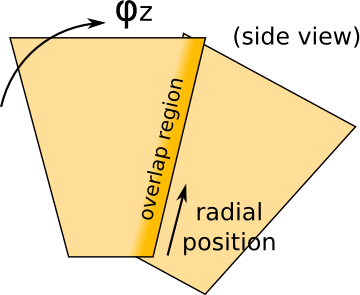
\includegraphics[width=\linewidth]{sideview.png}
\end{columns}
\end{frame}

\begin{frame}
\frametitle{Closure conditions}
\begin{itemize}
\item Four types of residuals, each measures a different parameter:

\renewcommand{\arraystretch}{1.3}

\begin{tabular}{c | c c}
& segment slopes & intercepts \\\hline
evaluated at center of chambers & $\varphi_y$ angles & $r\phi$ positions \\
linear trend versus radial position & chamber twist & $\varphi_z$ angles \\
\end{tabular}

\item No significant ``twist'' observed (shear of alignment pins)

\item Residuals measure chamber-by-chamber differences: in a ring, they must add to zero

\item All types of residuals add to zero (``close'') except $r\phi$

\item $r\phi$ residuals fail to close if chambers are the wrong width in \mbox{some sense:\hspace{-1 cm}}

\begin{itemize}
\item if the chambers are literally too wide or narrow
\item if the average distance to the beamline (radius) is wrong \\ (potentially measurable by closure, if we can rule out \mbox{other effects)\hspace{-1 cm}}
\item \sout{if chambers are rotated in $\varphi_y$} {\scriptsize (discussed in last DPG presentation)}
\end{itemize}

\item Last effect is second-order in $\varphi_y$, but we have a direct first-order measurement of $\varphi_y$ angles
\end{itemize}
\end{frame}

\begin{frame}
\frametitle{Status: last CMS Week}
\begin{itemize}
\item Only aligned $\varphi_y$ and $r\phi$ (and some $\varphi_y$ corrections \mbox{were questionable)\hspace{-1 cm}}
\item Wide residuals, presumed due to misaligned $\varphi_z$
\end{itemize}

\vfill
{\scriptsize Hollow: aligned (ME$-$2/1 \& $-$3/1 combined), grey: unaligned, \mbox{red line: ME$-$2/1-only fit\hspace{-1 cm}}}

\vspace{0.2 cm}
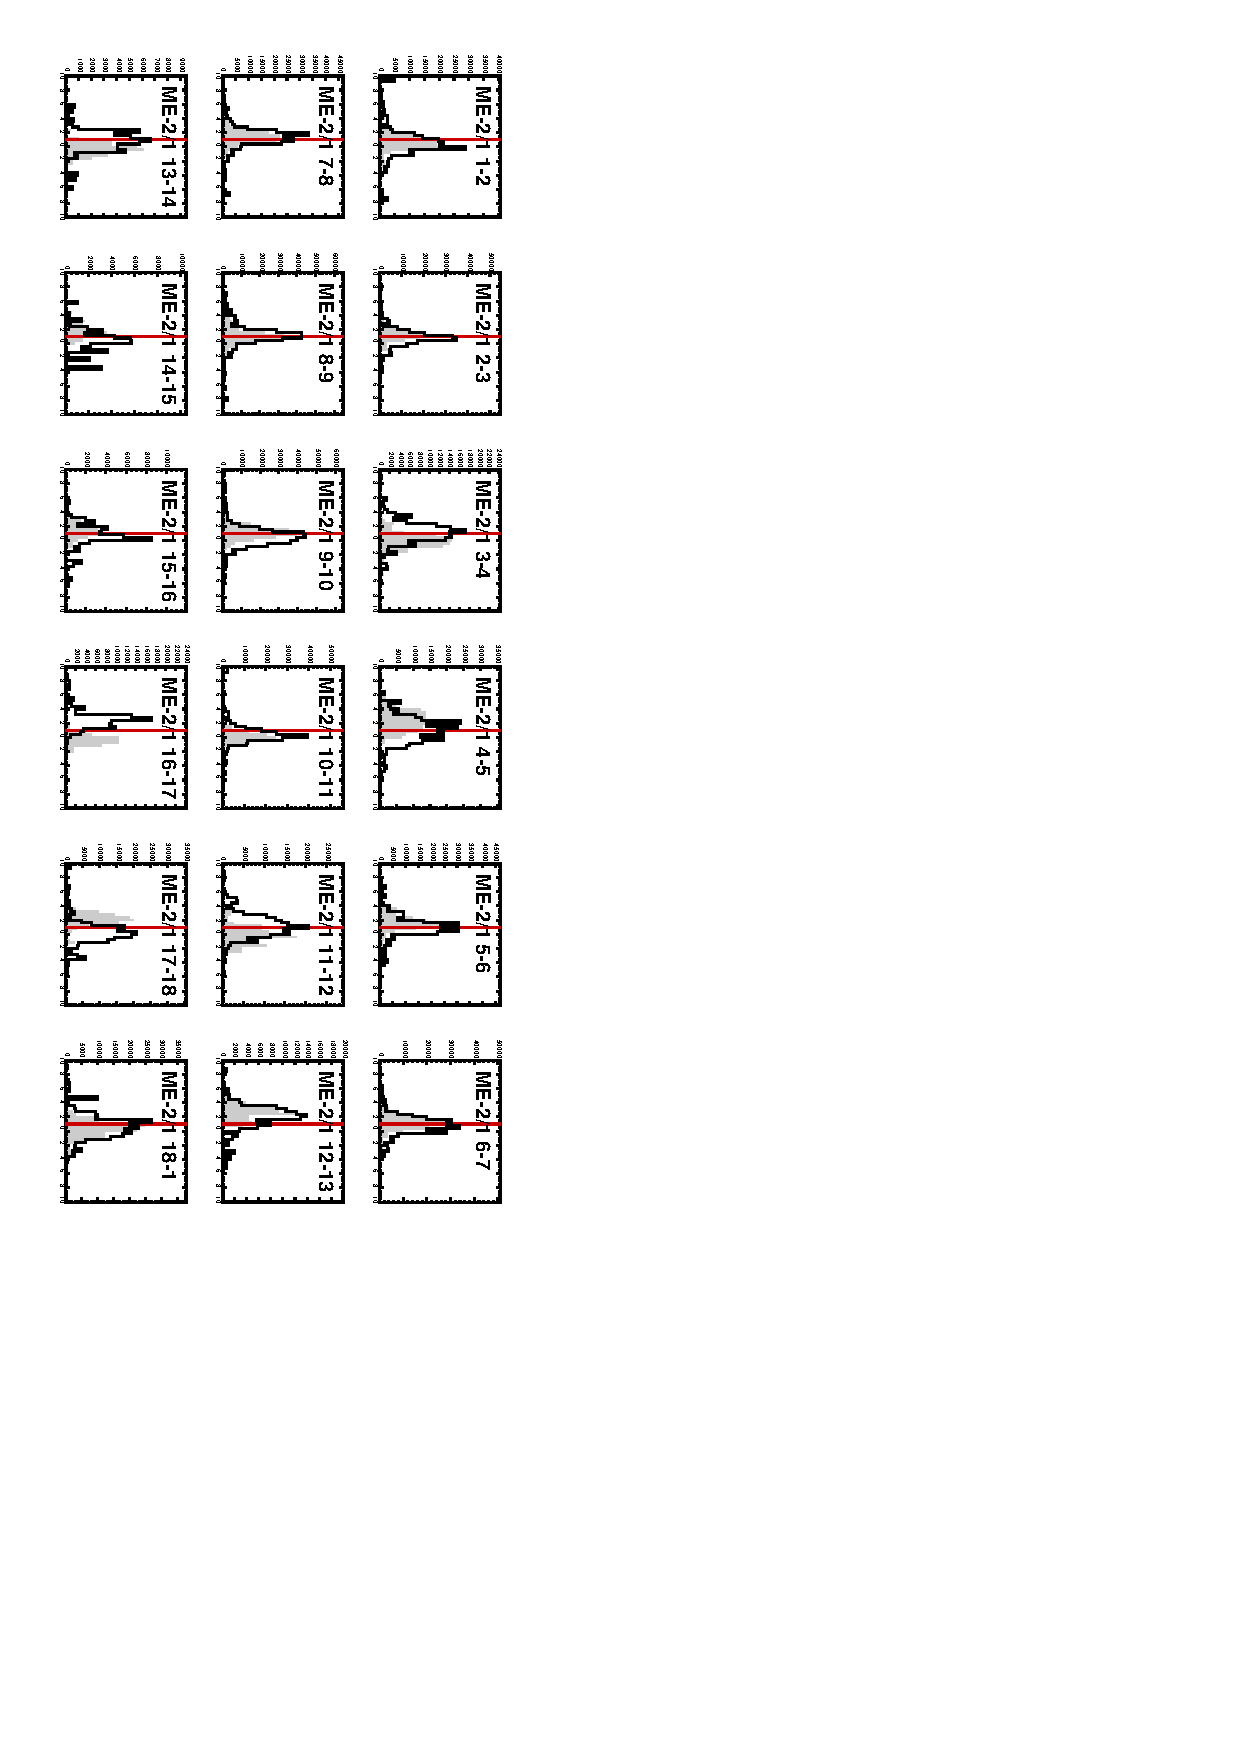
\includegraphics[height=\linewidth, angle=90]{final_checkresids_half.pdf}

\vfill
\begin{itemize}
\item ME$-$2/1, ME$-$3/1 whole-ring underclosure: 18~mm, 20~mm
\item Cross-checked overlaps alignment results against other track-based measurements (which are less precise than overlaps)
\end{itemize}
\end{frame}

\begin{frame}
\frametitle{Status: now}
\begin{itemize}
\item Full $\varphi_y$, $r\phi$, $\varphi_z$ alignment; intercept residuals are all 1.2~mm wide
\end{itemize}

\vfill
{\scriptsize Hollow: aligned (ME$-$2/1-only fit), grey: unaligned, red line: common mean}

\vspace{0.2 cm}
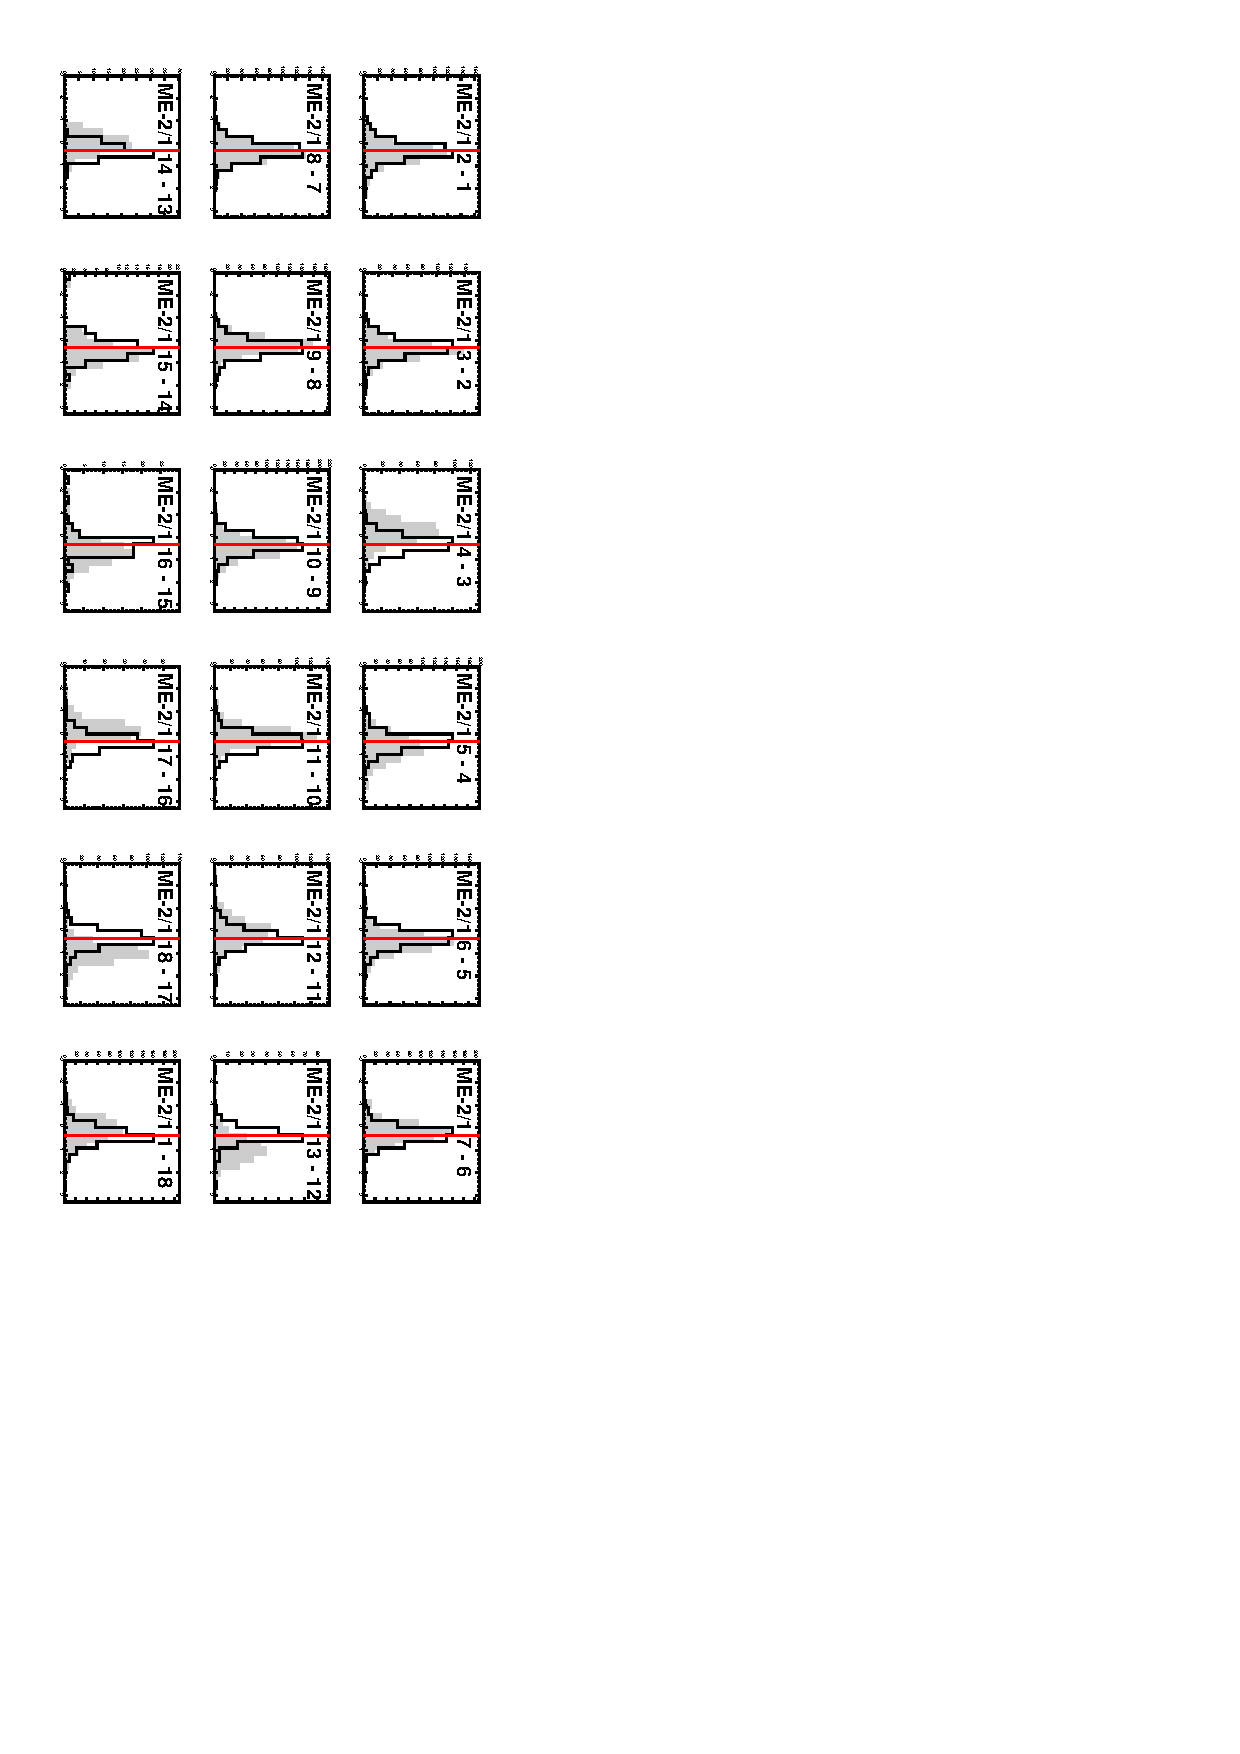
\includegraphics[height=\linewidth, angle=90]{residuals_hists_MEm21.pdf}

\vfill
\begin{itemize}
\item Used photogrammetry to set chamber-by-chamber distances from beamline: reduced underclosure by 20\%, but still significant
\item ME$-$2/1, ME$-$3/1 whole-ring underclosure: 16~mm, 14~$\pm$~0.4~mm
\item Interpreted as radial corrections: 2.5~mm, 2.3~mm inward
\item Cross-checked track-based alignment results \mbox{against photogrammetry\hspace{-1 cm}}
\end{itemize}
\end{frame}

\begin{frame}
\frametitle{Confidence in alignment results}

\begin{itemize}
\item The method is sound: Monte Carlo closure is consistent with zero
\item In data, all residual types have zero closure except $r\phi$
\item $r\phi$ and $\varphi_z$ constants compare favorably with photogrammetry
\end{itemize}

\only<1>{\scriptsize Overlay of $r\phi$ translations, track-based and photogrammetry relative to ideal}
\only<2>{\scriptsize Overlay of $\varphi_z$ rotations, track-based and photogrammetry relative to ideal}

\vfill
\only<1>{\hfill 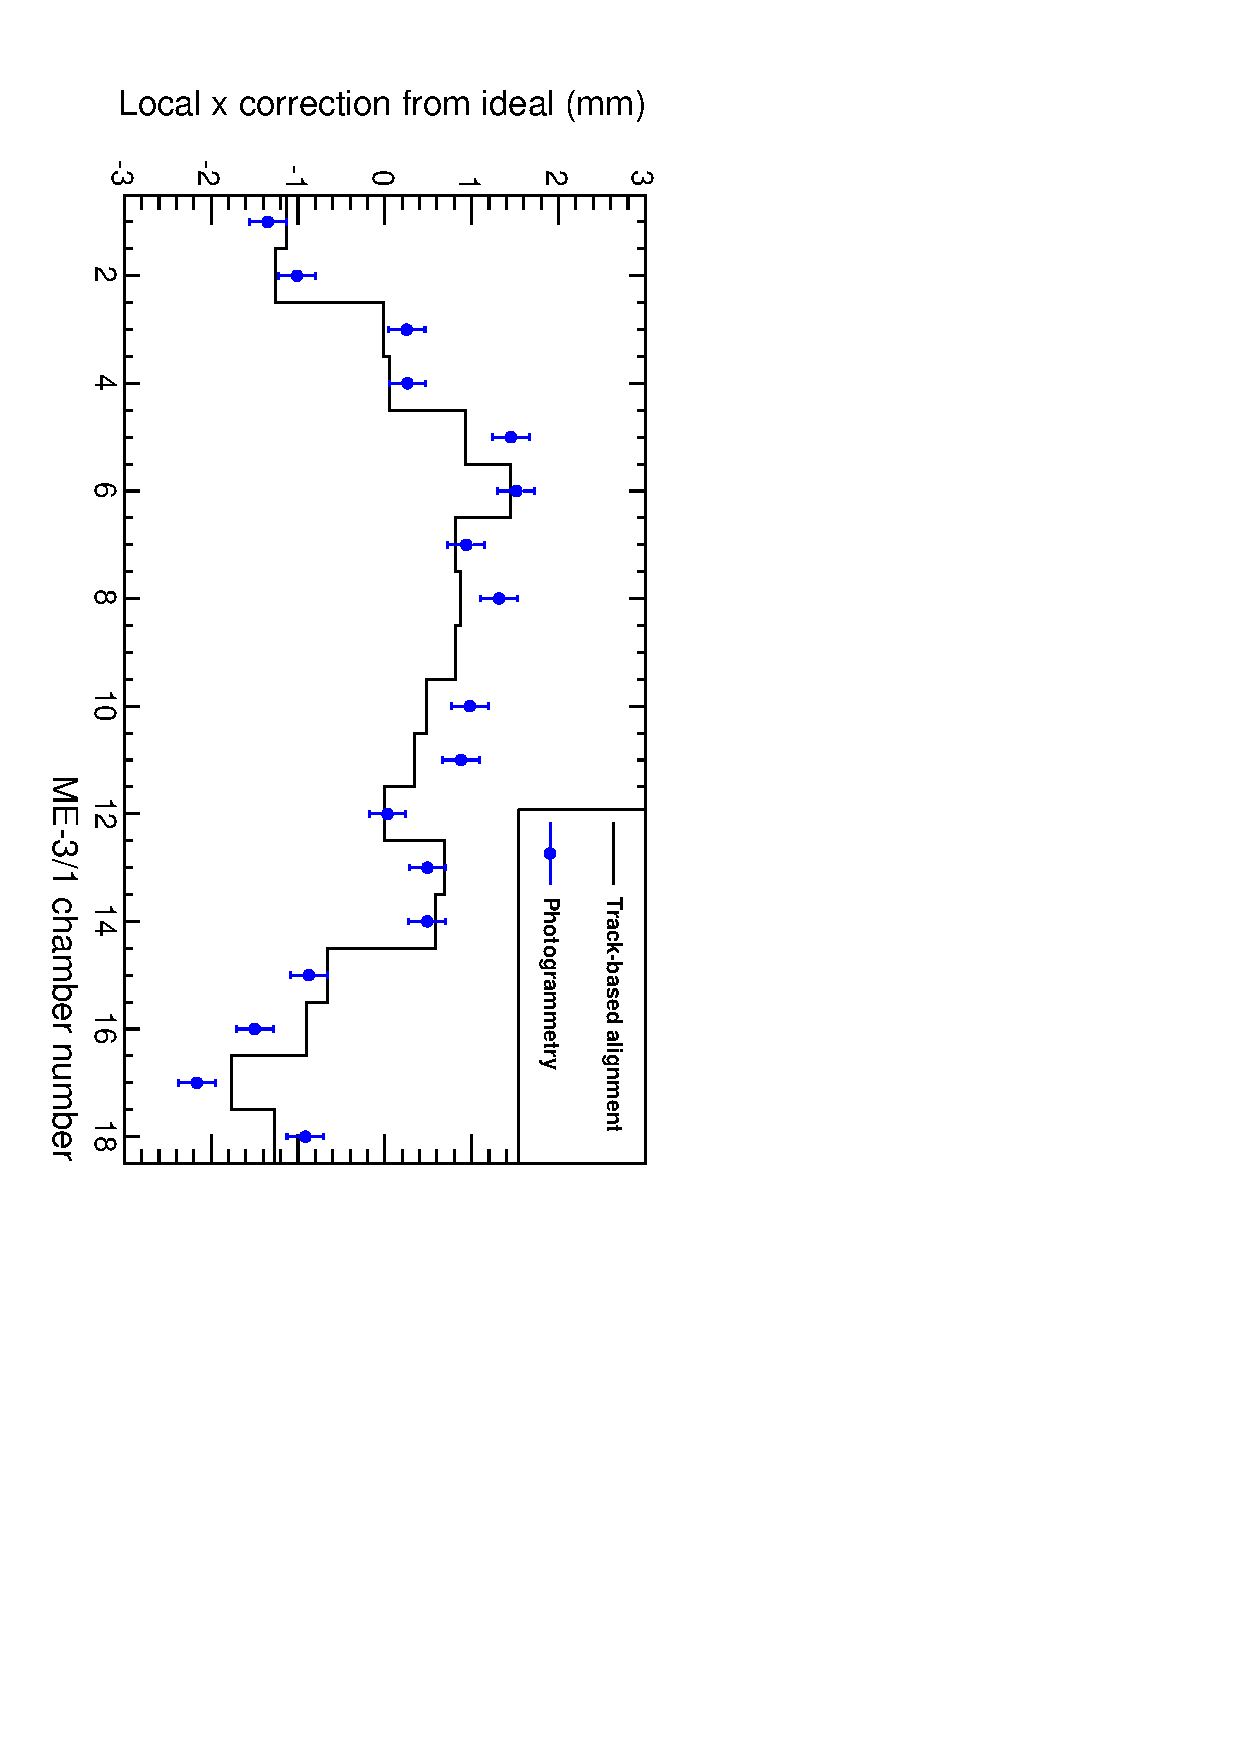
\includegraphics[height=0.95\linewidth, angle=90]{compare_m31_x.pdf} \hfill}
\only<2>{\hfill 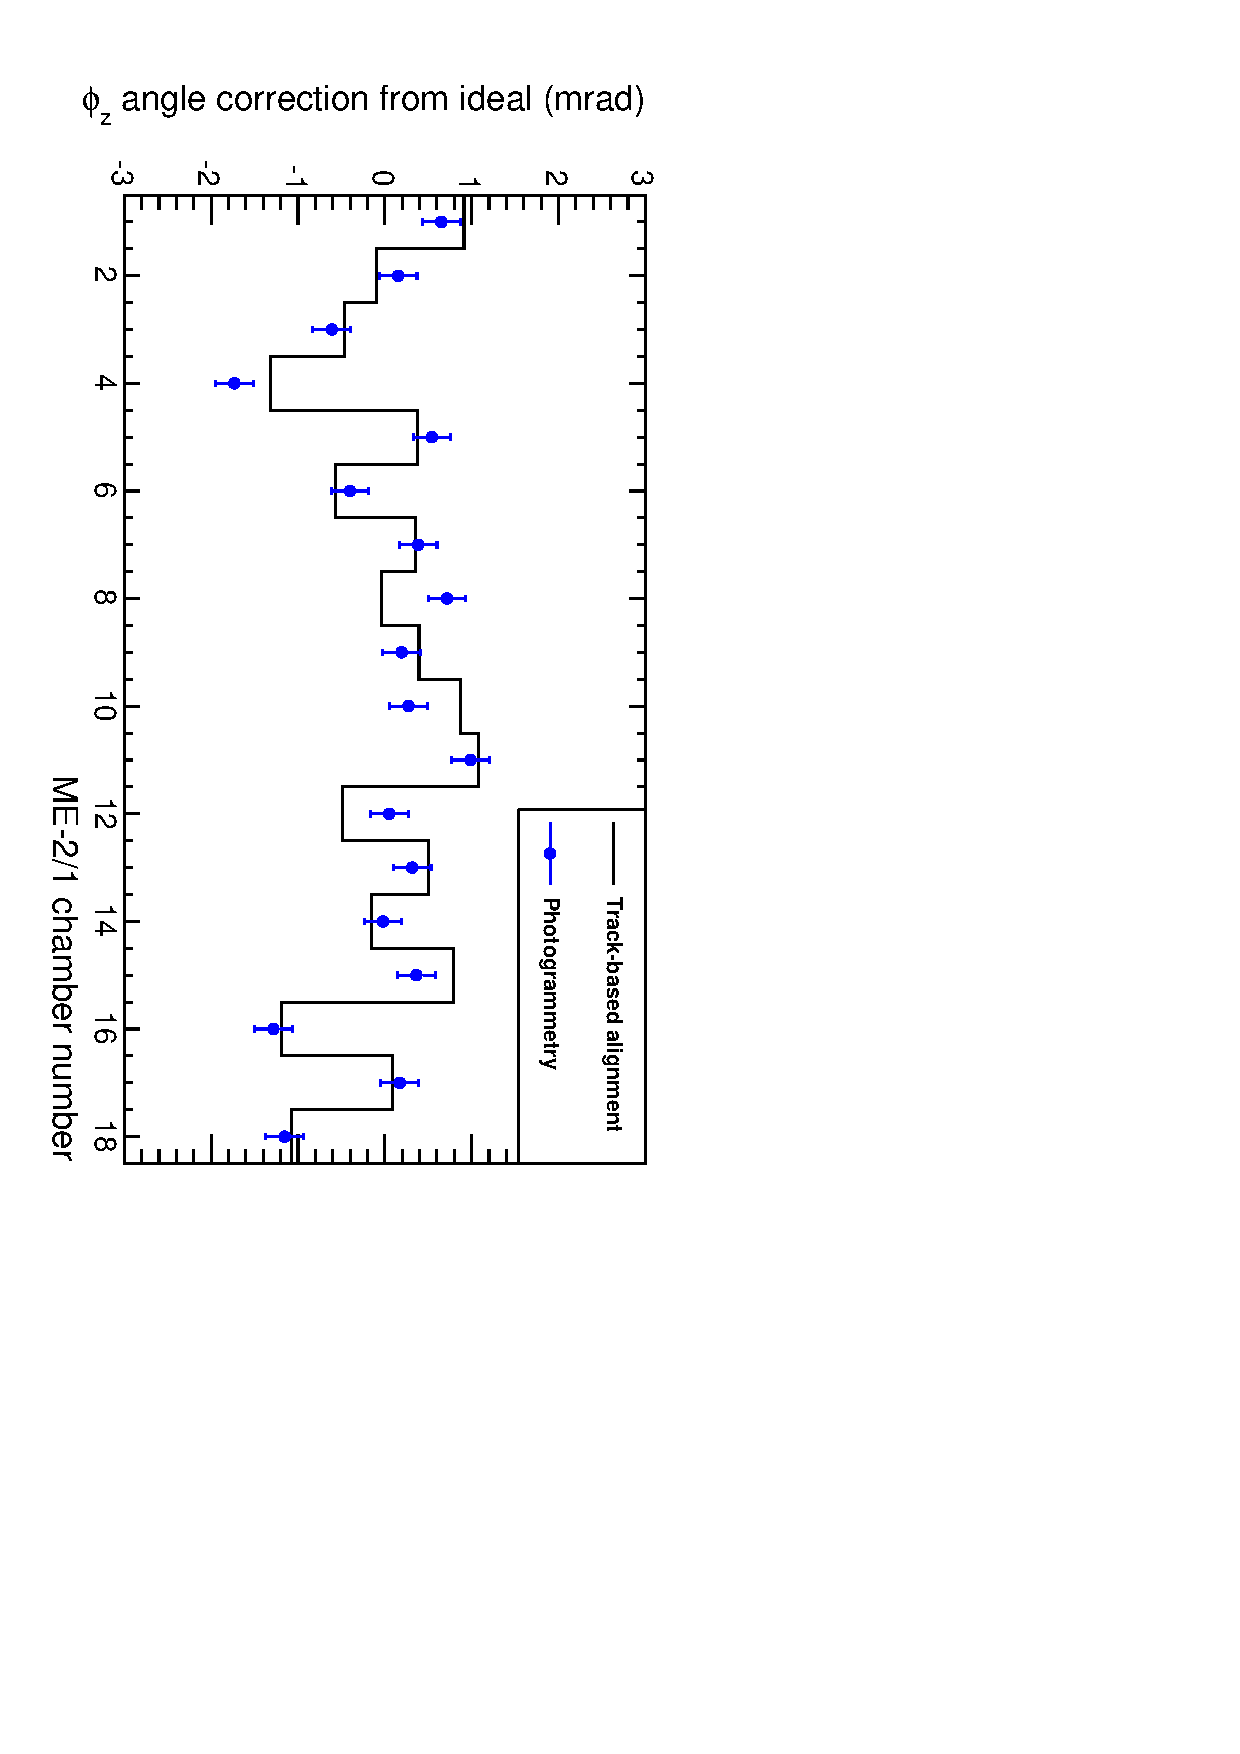
\includegraphics[height=0.95\linewidth, angle=90]{compare_m21_phiz.pdf} \hfill}
\end{frame}

\begin{frame}
\frametitle{Confidence in alignment results}
\begin{itemize}
\item RMS difference between track-based and PG: 340~$\mu$m, 0.42~mrad
\item Photogrammetry $r\phi$ uncertainty is (300/$\sqrt{2}$)~$\mu$m = 210~$\mu$m
\item $\sqrt{340^2 - 210^2}$ = \textcolor{red}{270~$\mu$m errors in track-based method alone}
\item Statistics from one large beam-halo run (62232, 9 minutes)
\end{itemize}

\begin{columns}
\column{0.5\linewidth}
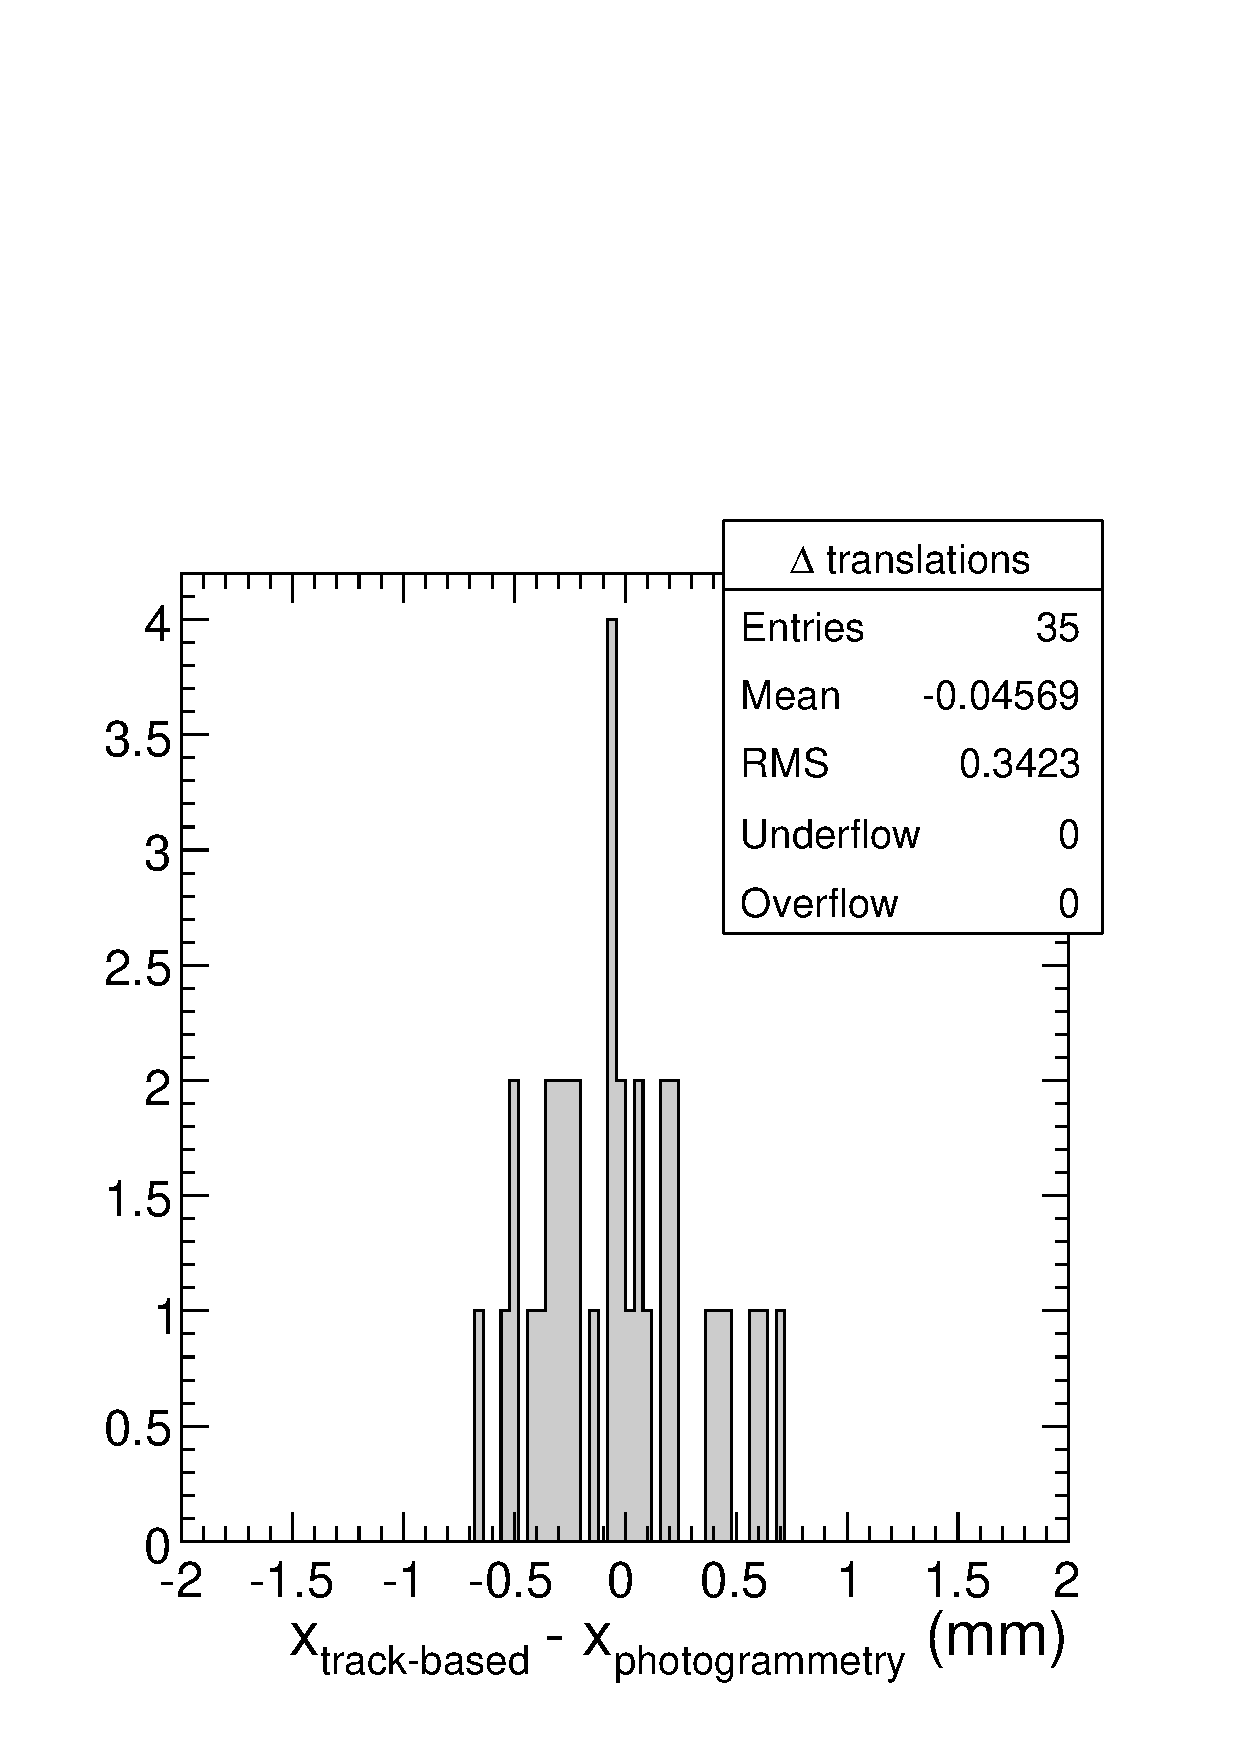
\includegraphics[width=\linewidth]{delta_translations.pdf}
\column{0.5\linewidth}
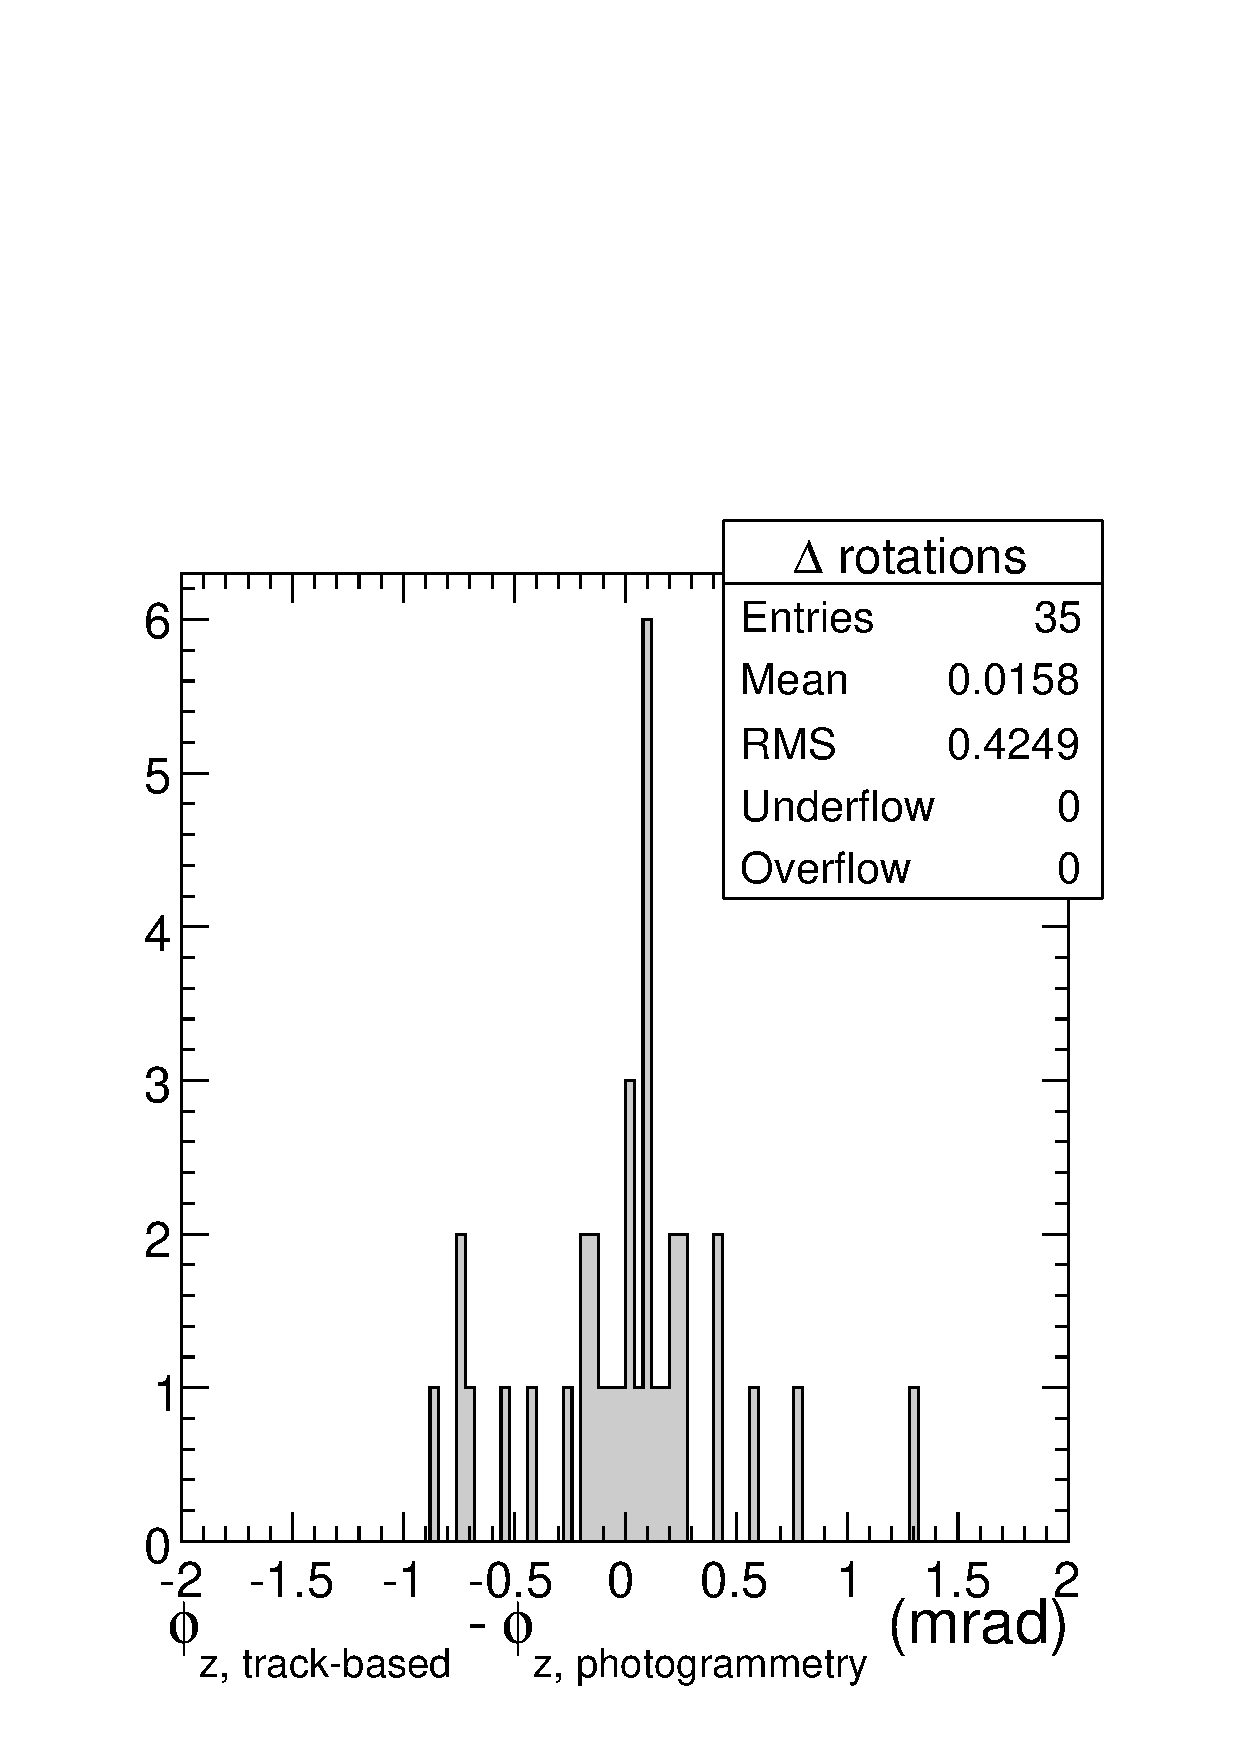
\includegraphics[width=\linewidth]{delta_rotations.pdf}
\end{columns}
\end{frame}

\begin{frame}
\frametitle{What about closure?}
\begin{itemize}
\item High-precision agreement with photogrammetry gives us confidence in alignment results (with closure error distributed uniformly)
\item Therefore, closure error is due to a systematic effect which is the same for each chamber
\item Are there trends versus $\phi$, radial position, or track slope?  No.
\end{itemize}

\vfill
\begin{columns}
\column{0.34\linewidth}
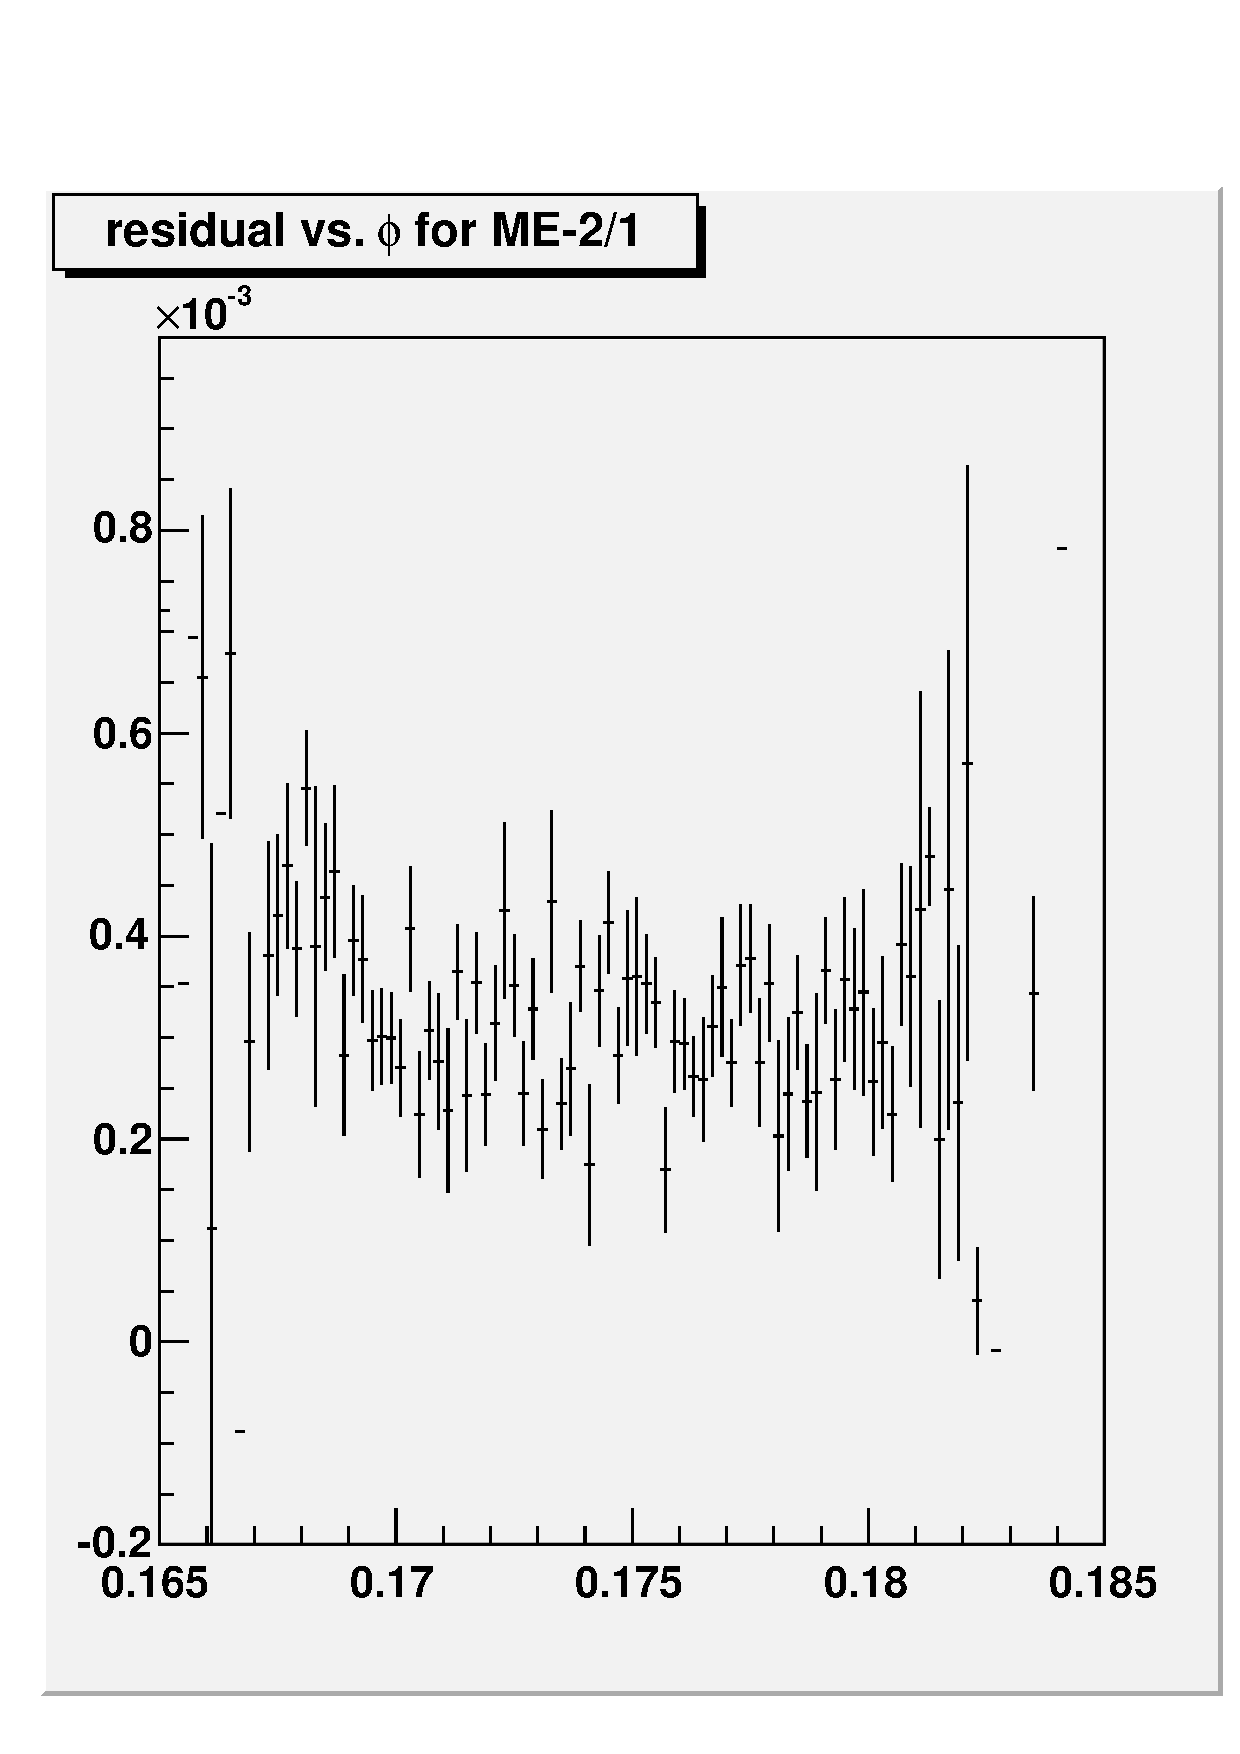
\includegraphics[width=\linewidth]{residual_vsphi.pdf}
\column{0.34\linewidth}
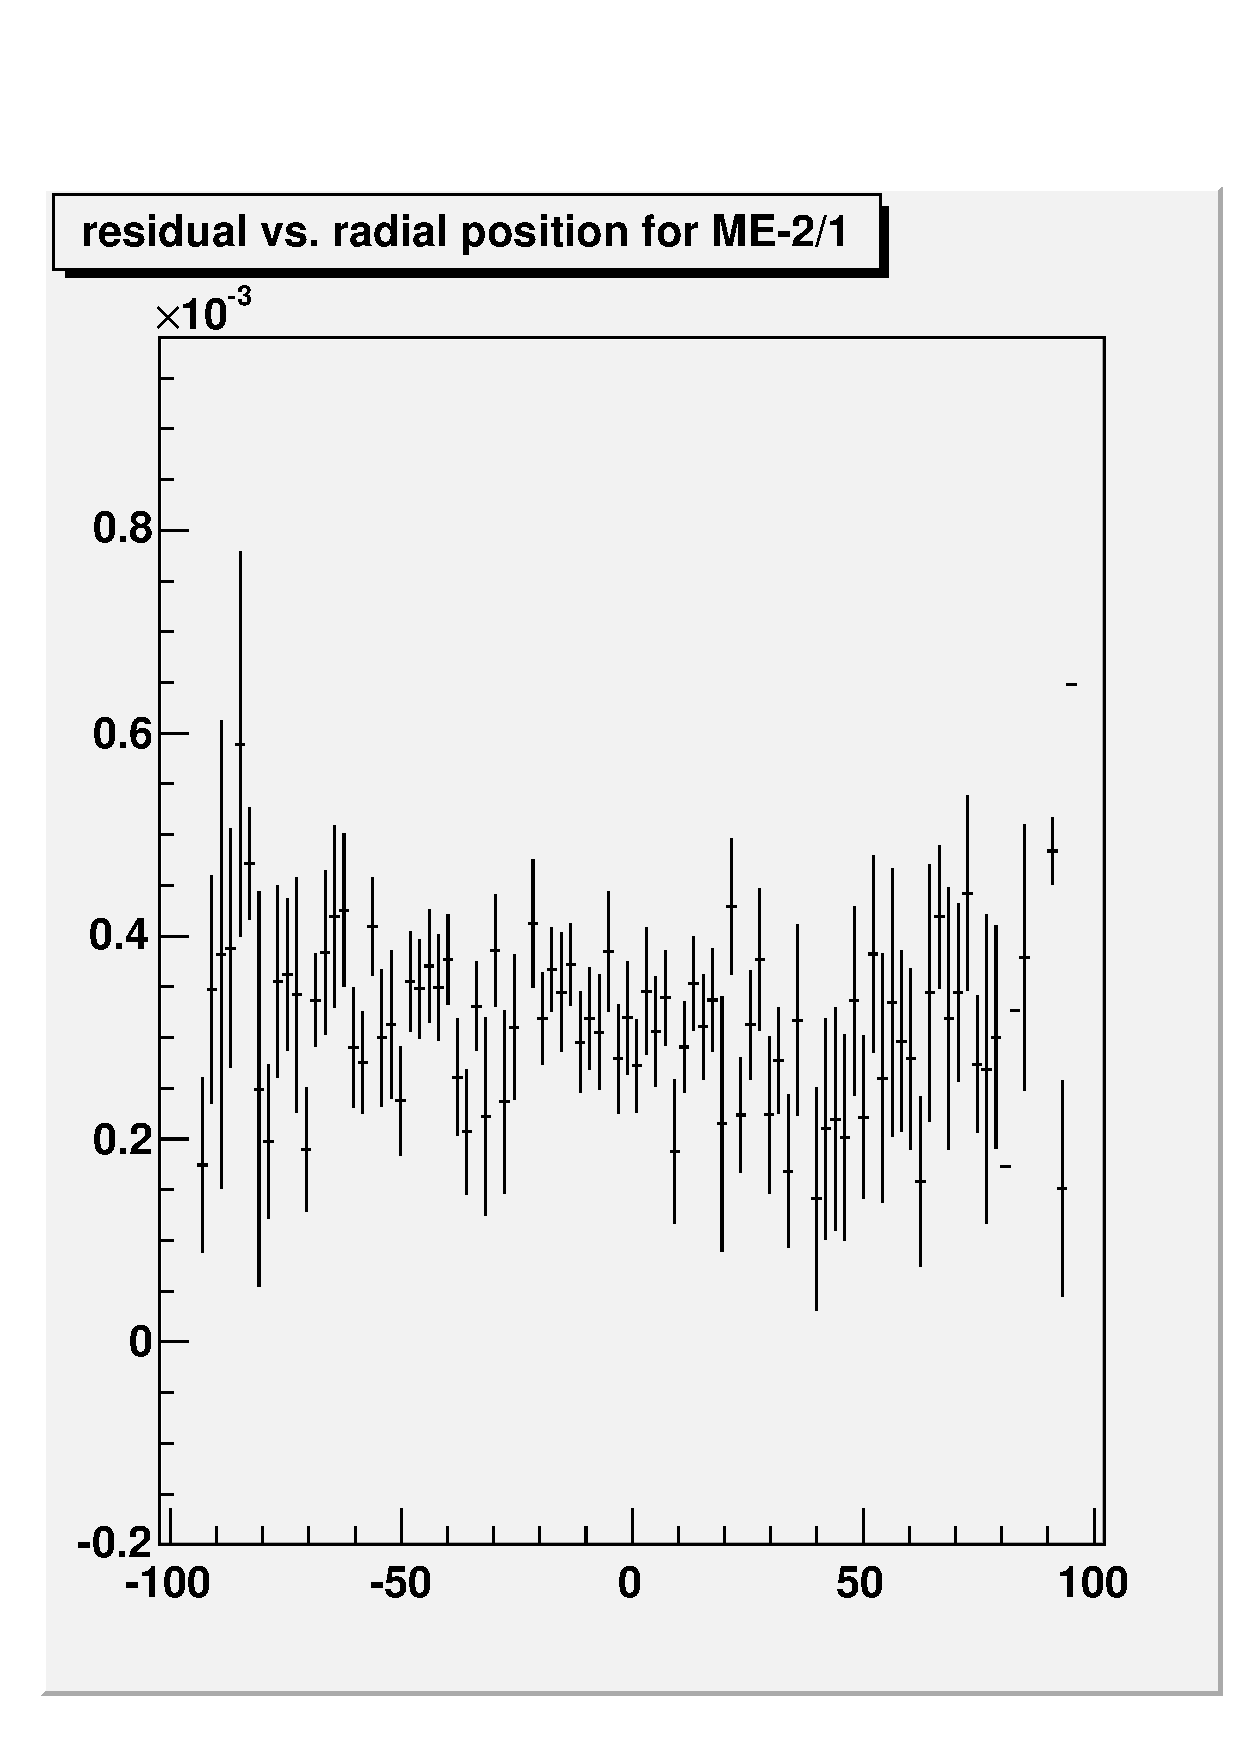
\includegraphics[width=\linewidth]{residual_vsradialpos.pdf}
\column{0.34\linewidth}
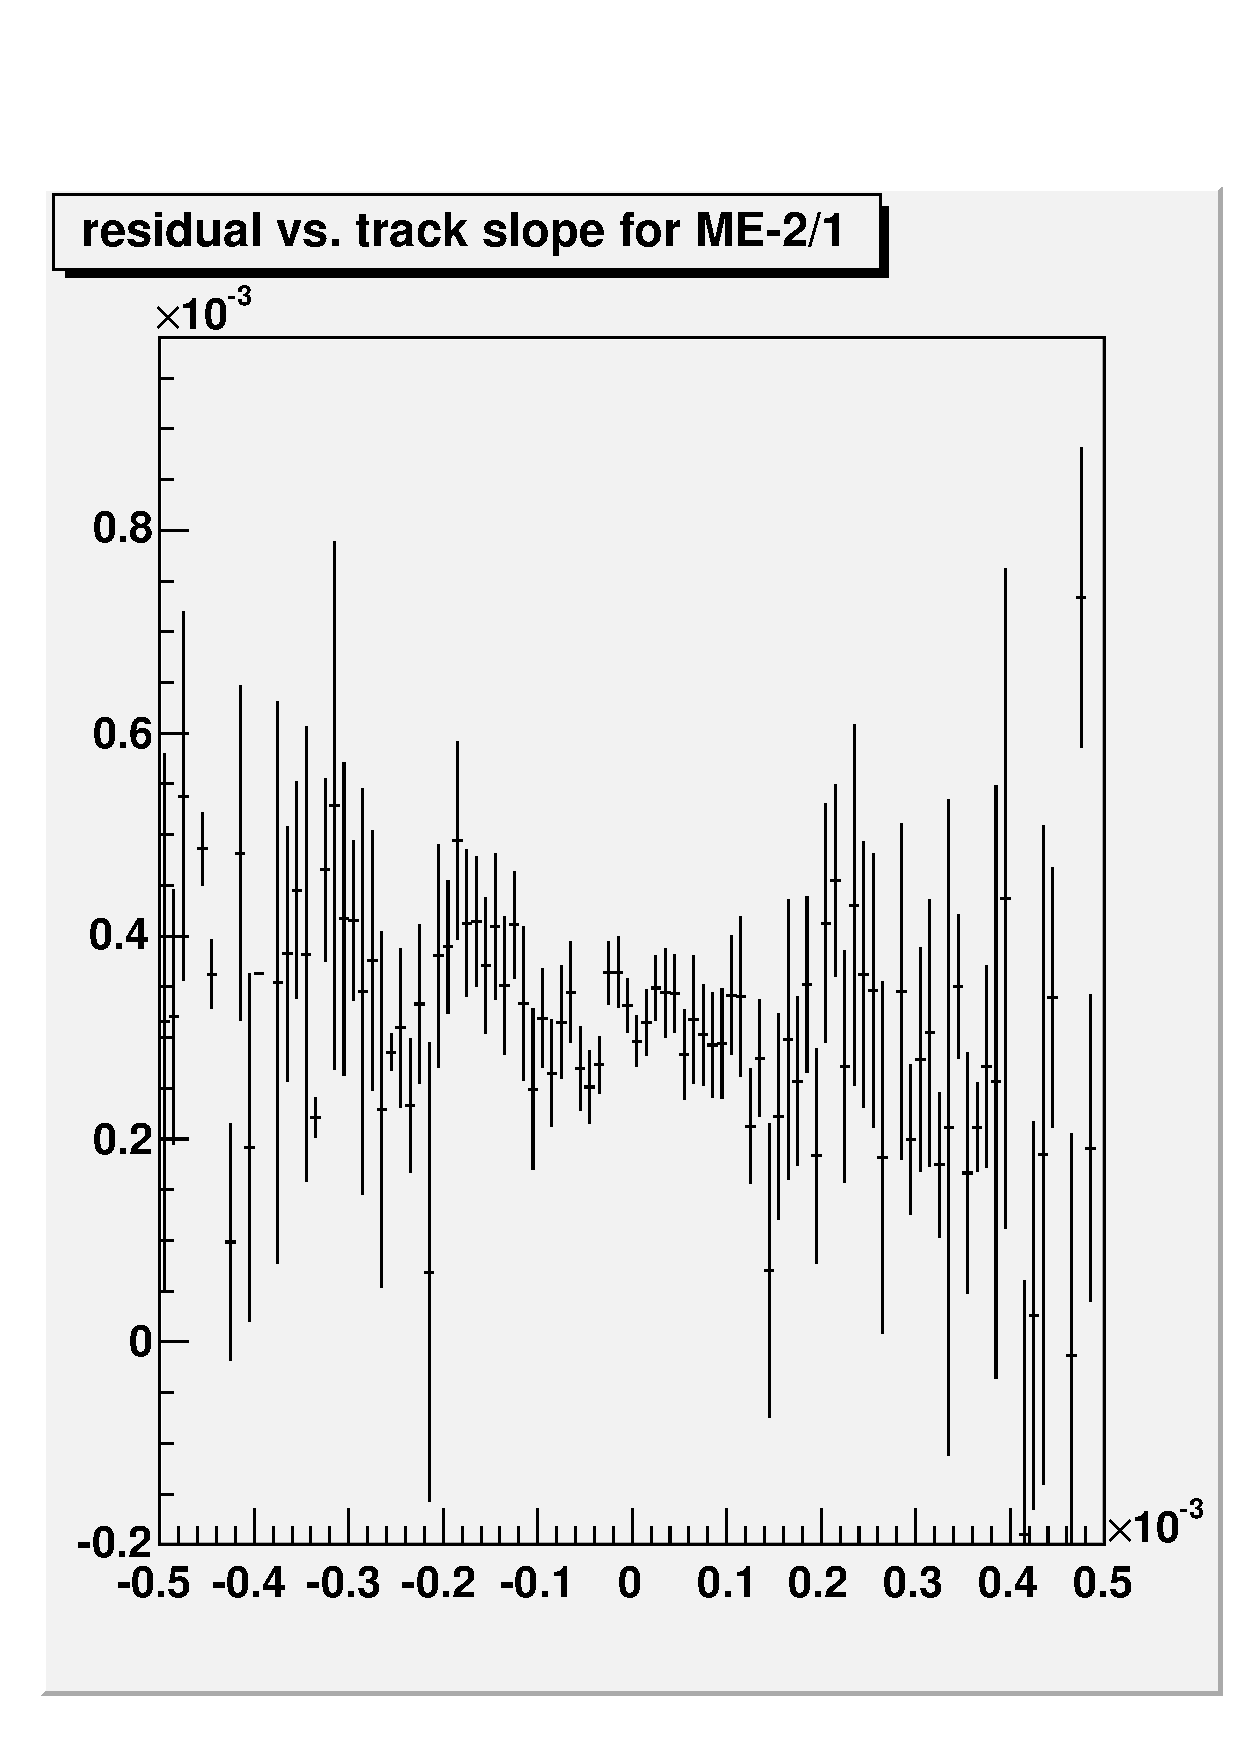
\includegraphics[width=\linewidth]{residual_vsslope.pdf}
\end{columns}
\end{frame}

\begin{frame}
\frametitle{Remaining possibilities}
\begin{itemize}\setlength{\itemsep}{0.2 cm}
\item \textcolor{darkblue}{Hypothesis 1:} layers are {\it narrower} in
  real life than in software by 0.8~mm at the center (0.087\% error in
  total width, or 10~$\mu$m \mbox{per strip)\hspace{-1 cm}}

\begin{itemize}
\item Maybe ``narrowing'' is due to bowing, e.g.\ if
  layer surface pinched to fit frame?  No: sagitta = 9.6~mm, bow angle = 4.8$^\circ$

\end{itemize}

\item \textcolor{darkblue}{Hypothesis 2:} chamber centers are {\it
  closer} to the beamline by 2.5~mm in ME$-$2/1 and 2.3~mm in ME$-$3/1 ($\pm$ 0.06~mm each)

\begin{columns}
\column{0.04\linewidth}

\column{0.7\linewidth}
\begin{itemize}
\item We've verified the alignment pin positions \mbox{in $\phi$, and can\hspace{-2 cm}}
  therefore be certain that they are correct in $r$ (photogrammetry
  errors must be isotropic in $x$ and $y$!)
\item Therefore, we're not disputing the global pin positions, but the
  chamber centers relative to those pin positions \mbox{(from mf.xml)\hspace{-1 cm}}
\item Also, this is not the chamber center as measured by the wires
  (the normal way of measuring radial position), \mbox{but measured through angle of strips\hspace{-4 cm}}
\end{itemize}

\column{0.005\linewidth}

\column{0.3\linewidth}
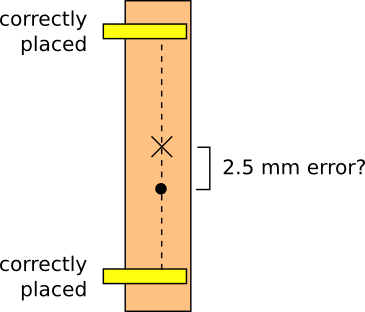
\includegraphics[width=\linewidth]{pins_are_okay.png}
\end{columns}
\end{itemize}
\end{frame}

\begin{frame}
\frametitle{Ideas to search for the effect}

\begin{itemize}\setlength{\itemsep}{0.1 cm}
\item It was a {\it different} 2.5~mm offset that we found a few months ago
  by looking at the drawings (ME2/2 and 3/2, and in opposite direction)

\item We didn't see an analogous effect in other rings, but there
  might be a different drawing/DDD discrepancy, e.g.\ distance from
  pins to center, rather than bottom of chamber frame to center

\item Track-based method to cross-check hypothesis \#2 (radial shift):
  wire residuals or strip efficiency turn-on curve (more direct)
\end{itemize}

\vfill
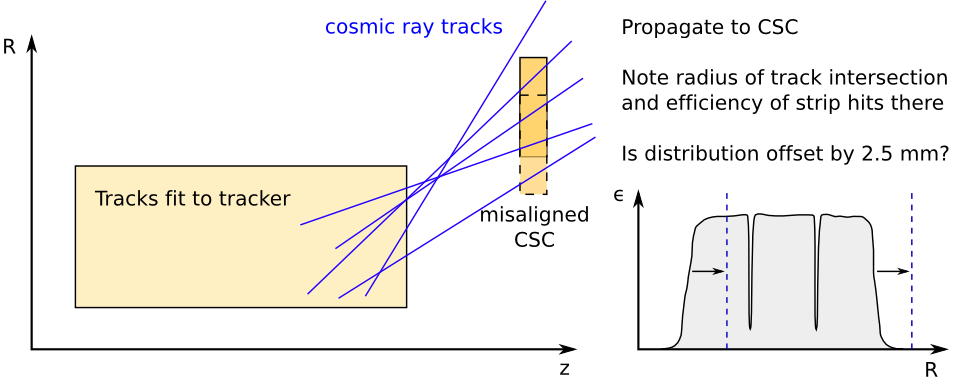
\includegraphics[width=\linewidth]{way_to_find_radial_misalignment.png}
\end{frame}

%% \section*{First section}
%% \begin{frame}
%% \begin{center}
%% \Huge \textcolor{blue}{First section}
%% \end{center}
%% \end{frame}

\begin{frame}
\frametitle{Conclusions}
\begin{itemize}\setlength{\itemsep}{0.5 cm}

\item Our alignment results are correct, to desired precision (300~$\mu$m)

\item However, $r\phi$ residuals very clearly do not close when summed around rings ME$-$2/1 and ME$-$3/1

\item The problem is uniform across all these chambers: if it were
  not, we would not be able to reproduce photogrammetry

\item Real chambers are \underline{\mbox{\hspace{1 cm}}} than in simulation
\begin{itemize}\setlength{\itemsep}{0.1 cm}
\item 0.8~mm narrower across the center
\item 2.4~mm closer to the beamline
\item \sout{pinching layers such that they bow by 4.8$^\circ$ more}
\item \sout{50-70$^\circ$ C colder}
\item or\ldots?
\end{itemize}

\end{itemize}
\label{numpages}
\end{frame}

\end{document}
